\chapter{Scalability And Hyperparameter Optimization}
\label{chap:scalability}

\newepigraph{While we cannot accurately predict the course of climate change in the coming decades, the risks we run if we don't change our course are enormous. Prudent risk management does not equate uncertainty with inaction.}{Steven Chu}

The previous chapters focused in forecasting tasks and its uncertainties and FTS approaches were presented to deal with theses issues. However, the presented approaches do not optimize its models for a given time series $Y$. The best hyperparameters must be found by the user and then informed to the methods, task that was delegated until now to an expensive Grid Search optimization.

As reviewed in Chapter \ref{chap:review_fts}, several approaches in the literature embody optimization tasks in their training procedures. Nevertheless an holistic hyperparameter optimizer for all FTS components present in Table \ref{tab:fts_hyperparameters} is still lacking in the literature. The most challenging issue presented by this task is the choose of the partitioning method $\Pi$, which may use computationally expensive meta-heuristics (and without known parallel or distributed extensions), and the number of partitions $k$ and order $\Omega$ that regulates the parsimony of the model.

The optimization task becomes even harder when dealing with time series with Big Data properties. Many of the traditional forecasting methods, and even some new ones, were not designed to deal with such high volume of data. The most critical issues are the high dimensionality (dozens of hundreds of attributes) and volume (hundreds of millions or billions of samples), as pointed out in \cite{Qiu2016}. There is not a universal consensus about the small, medium and big data sizes. By simplicity it can be considered that it strongly depends on the available hardware capabilities. 

In all cases Big Data starts to happen when it does not fit in the memory of a single machine. Such data volume, that cannot be grounded on a single machine memory, demands a distributed architecture of storage and processing. New technologies are emerging to tackle these issues, for instance the Map Reduce based frameworks \cite{Dean2008}, a  divide-and-conquer approach which is the basis of Hadoop clusters \cite{White2012}, where the processing units also act as storage units of the data subsets. 

These distributed computation approaches have been determinant to enable the processing of data-intensive and computationally expensive tasks. Thanks to the distributed computation frameworks, soft-computing methods are now enabled to work with massive datasets using cheap and available hardware infrastructure. Such kind of tasks are spread over several areas in science and engineering, such as in weather and environmental datasets and on smart sensor data of smart grids where, according to \cite{Coelho2016}, there are networks of smart sensors continuously monitoring all system components and streaming historical data with high volume and velocity. 

Applying Big Data to machine learning algorithms is a trending topic in recent years, as can be seen in \cite{Zhou2017}. But the literature on taming big time series did not considered FTS methods directly, although there exists approaches involving other fuzzy methods, see for instance \cite{Singh2015}.

The absence of computationally expensive iterative procedures inside the training and forecasting procedures of the proposed FTS methods facilitates its scalability, as well as the use of white box knowledge models that can be easily distributed and updated. With this design, FTS models $\model$ can be quickly trained in commodity hardware, without major processing requirements, and transferred between cluster nodes. 

This chapter aims to propose scalable alternatives to perform  training FTS methods using distributed algorithms and exploit  these solutions to tackle the hyperparameter optimization of big time series. In Section \ref{sec:distributed} an distributed FTS training approach for big time series is proposed. In Section \ref{sec:hyperparameter} the Distributed Evolutionary Hyperparameter Optimization (DEHO) method is proposed, combining evolutionary algorithms and the previously defined distributed training and forecasting approaches. In Section \ref{sec:scalability_experiments} computational experiments are performed to assess the speed up provided by the distributed methods and the convergence of DEHO method for large environmental time series. Finally, in Section \ref{sec:scalability_conclusion} the results are discussed and synthesized.

%%%%%%%%%%%%%%%%%%%%%%%%%%%%%%%%%%%%%%%%%%%%%%%%%%%%%%%%%
%%%%%%%%%%%%%%%%%%%%%%%%%%%%%%%%%%%%%%%%%%%%%%%%%%%%%%%%%
\section{Computational Clusters}

According to \cite{Baker1999}, ``A cluster is a type of parallel or distributed processing system, which consists of a collection of interconnected stand-alone computers working together as a single, integrated computing resource''. Clusters are used for providing high availability, load-balancing, distributed storage, high processing power, among other purposes.

The Distributed Storage Clusters (DSC) systems are employed to keep distributed database systems or distributed file systems, exploiting local storage resources to allow the storage of data volumes that can be handled by a single machine, while providing transparent access to the whole dataset. Diversely, the High Processing Clusters (HPC) systems are employed to solve complex or expensive computational tasks which can be decomposed and parallelized by sub-datasets (Single Instruction / Multiple Data), sub-tasks (Multiple Instruction / Single Data) or both (Multiple Instruction / Multiple Data). A good example of HPC cluster is the classical Beowulf Cluster\footnote{The Beowulf Project - \url{http://www.beowulf.org}. Access in 15/05/2019} architecture, which makes use of message passing middleware like MPI and PVM. In these frameworks the instructions and data are spread across the cluster and, after the local processing on each cluster node finishes, the results are gathered in some master or control node. 

With the advent of Big Data, the demand of distributed file systems capable to store large datasets was joined with the demand for simple programming interfaces for processing distributed data. The Map/Reduce, proposed in \cite{Dean2008}, became a popular distribution paradigm due to its high adoption in Big Data literature. In such paradigm the computational cluster contains a master node, which centralizes the management of the tasks, and several slave nodes responsible for working tasks. The distributed execution is divided into two main phases, the map (scattering) and reduce (gathering). The Map phase splits the original dataset into smaller subsets and distributes them to the slave nodes. Each individual slave node will perform the same predefined set of computations on data and send the results back to the master node. The Reduce phase collects the results from the slave nodes and performs final aggregations of results.

The popularity of the Map/Reduce paradigm to tackle Big Data problems imersed after the first open source infrastructure frameworks became available, for instance Apache Hadoop\footnote{Apache Hadoop Project - \url{https://hadoop.apache.org/}. Access in 15/05/2019}. More recently some infrastructure was developed to allow in-memory processing, turning the processing yet more efficient, as for instance the Spark framework\footnote{Apache Spark - \url{https://spark.apache.org/}. Access in 15/05/2019}. In the next sections, the distribution strategies for the sequential FTS methods are discussed using HPC middleware and Map/Reduce paradigm.


%%%%%%%%%%%%%%%%%%%%%%%%%%%%%%%%%%%%%%%%%%%%%%%%%%%%%%%%%
%%%%%%%%%%%%%%%%%%%%%%%%%%%%%%%%%%%%%%%%%%%%%%%%%%%%%%%%%
\section{Scalable Models With Distributed Execution}
\label{sec:distributed}

Depending on the data size and the capabilities of the available infrastructure, different approaches must be considered for FTS method scalability, specially when dealing with hyperparameter optimization.

Small-sized time series (up to 10,000 instances) can be handled easily by a single machine and the costs of distribution (network and middleware overhead) do not pay off. This is the approach presented in all previous chapters.

For middle sized data (from 10,000 to 500,000 instances) the optimization process is more likely task-intensive, the evaluation dataset $Y$ can be split in smaller train/test data windows that can be handled by a single machine, and just the accuracy results need to be gathered and agregated. This is the approach presented in Section \ref{sec:distributed_testing}.

However, for highly sized data (above 500,000 instances), even the train/test data windows are costly to be trained by a single machine. In this case the training and testing methods need to be distributed themselves. This is the approach presented in Section \ref{sec:distributed_models}.



%%%%%%%%%%%%%%%%%%%%%%%%%%%%%%%%%%%%%%%%%%%%%%%%%%%%%%%%%
%%%%%%%%%%%%%%%%%%%%%%%%%%%%%%%%%%%%%%%%%%%%%%%%%%%%%%%%%
\subsection{Distributed Testing With Sequential Models}
\label{sec:distributed_testing}

The distributed testing with sequential models aims to speed up iterative optimization processes that require unnumbered evaluations of the objective function with different small to medium datasets. Each evaluation requires a sample of the entire dataset with which an FTS model $\model$ will be trained and evaluated using an accuracy metric $\epsilon$.

This is particularly the case of the hyperparameter optimization where, given a set of hyperparameters $\Theta$ and a time series dataset $Y$, for each combination of hyperparameters values $\theta \in \Theta$ being evaluated, it must perform a rolling window cross validation on the time series dataset. The distributed rolling window cross validation, shown in Figure \ref{fig:distributed_testing}, splits the whole dataset $Y$ in $W$ smaller and overlapping data windows $i=1..W$ and each data window is divided in train and test subsets. Then, for each data window $i$, a new model $\model_i$ will be trained and evaluated, generating the local accuracy metric $\epsilon_i$. The average of the accuracy metric is calculated as $\epsilon = W^{-1} \sum_{i=1}^W \epsilon_i$.

\begin{figure}[htb]
    \centering
    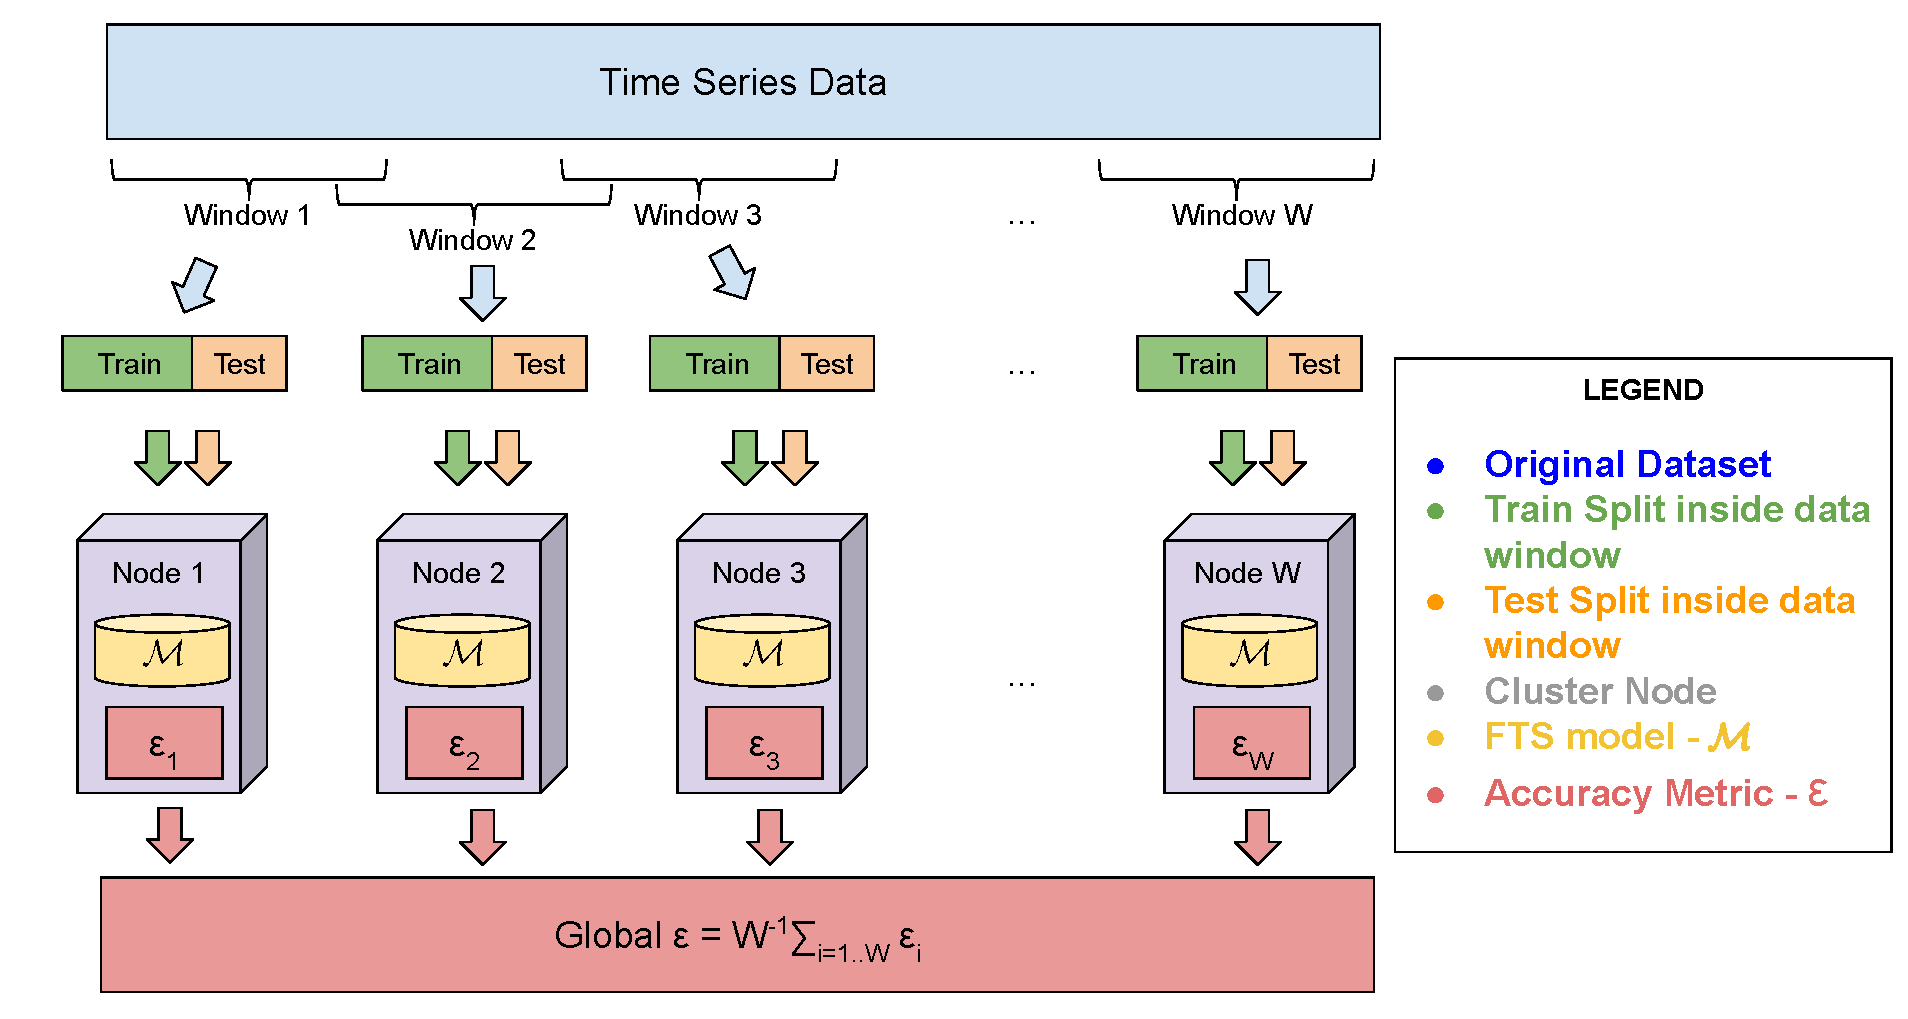
\includegraphics[width=\textwidth]{figures/distributed_testing.pdf}
    \caption{Distributed Testing With Sequential Models approach}
    \label{fig:distributed_testing}
\end{figure}

\begin{table}[htb]
    \centering
    \begin{tabular}{|c|c|p{7cm}|} \hline
        \textbf{Parameter} & \textbf{Name} & \textbf{Description} \\ \hline
         $0 < W_L < |Y|$ & Window Length & the number of time series instances in each data window \\ \hline
         $W_I \in [0,1]$ & Window Increment & Percentage of $W_L$ which is used to move the window \\ \hline
         $T_S \in [0,1]$ & Train/Test split & Percentage of $W_L$ which is used as training set and the remaining as test set.  \\ \hline
    \end{tabular}
    \caption{Distributed Testing Parameters}
    \label{tab:distributed_testing}
\end{table}

The distributed testing uses the parameters in Table \ref{tab:distributed_testing}. The number of data windows $W$ is given by $W = \max \{w\; |\; w(W_L\cdot W_I) + W_L \leq |Y| \}$ where $|Y|$ is the length of $Y$, and the process illustrated in Figure \ref{fig:distributed_testing} is executed in each evaluation of optimization engine. The key advantage of this approach is that it does not require any change on the FTS training and testing methods, just an adaption in the way the optimizer performs the evaluations. 

However, for big time series it is not enough. Depending on $|Y|$ and the capabilities of the available hardware, choosing of $W_L$ and $W_I$ may lead to three scenarios: a) $W_L$ will be larger than the available memory of the cluster nodes; b) a value of $W$ much greater than the number of cluster nodes, implicating in several rounds of computation for each node; c) $W_I$ too large that leads to the sub-sampling of the data (the windows are not overlapped and let ranges without been tested). None of these scenarios is desirable and thus a new approach must be considered.

%%%%%%%%%%%%%%%%%%%%%%%%%%%%%%%%%%%%%%%%%%%%%%%%%%%%%%%%%
%%%%%%%%%%%%%%%%%%%%%%%%%%%%%%%%%%%%%%%%%%%%%%%%%%%%%%%%%
\subsection{Distributed Models}
\label{sec:distributed_models}

For big time series the choosing of $W_L$ and $W_I$ values that do not lead to sub-sampling or cluster overhead, may fatally lead to a value of $W_L$ greater than the available machine memory. In this case even the windows must be split in smaller ones and the methodology of training and testing the models must change. Several stages of the training processes defined in Sections \ref{sec:fts_training_procedure} and  \ref{sec:pwfts_training} can be executed in parallel or distributed, on a Single Instruction/Multiple Data (SIMD) approach, since the data splits preserve the inherent time ordering. This characteristic allows the procedure's distribution to enhance their scalability and enable it to handle big time series.

This new approach changes the training method to first run the sequential procedure on individual cluster nodes with a slice of the original data window, creating a sub-model $\model_i$. Then the locally trained models are transmitted back to a master node where all local models are merged in a unique global model $\model$, as illustrated in Figure \ref{fig:distributed_models}. In the next sections the distributed training and forecasting methods are presented.

\begin{figure}[htb]
    \centering
    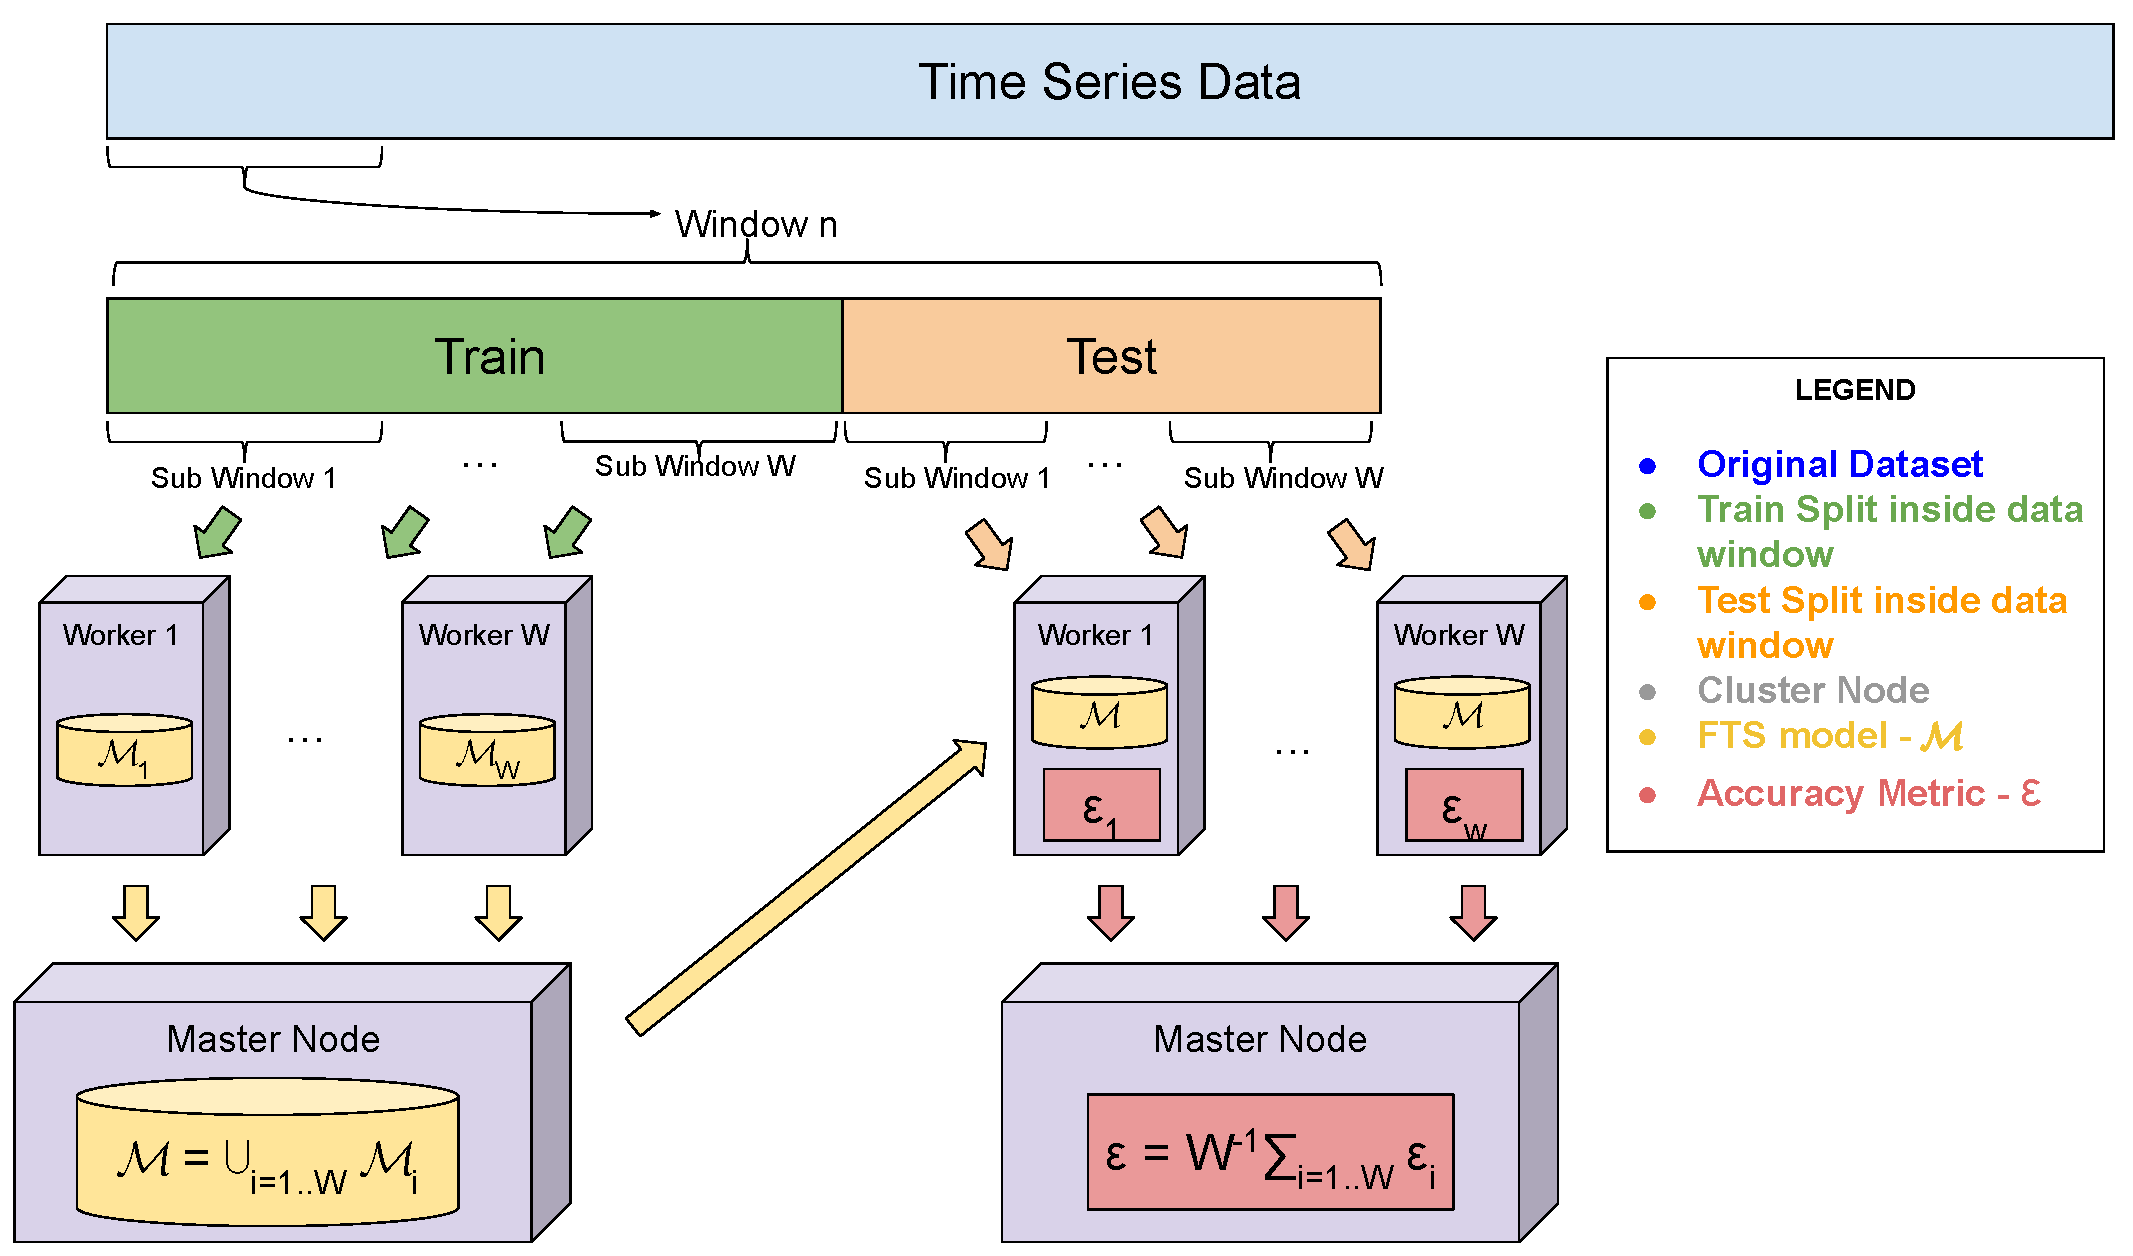
\includegraphics[width=\textwidth]{figures/distributed_models.pdf}
    \caption{Distributed Models approach}
    \label{fig:distributed_models}
\end{figure}


%%%%%%%%%%%%%%%%%%%%%%%%%%%%%%%%%%%%%%%%%%%%%%%%%%%%%%%%%
%%%%%%%%%%%%%%%%%%%%%%%%%%%%%%%%%%%%%%%%%%%%%%%%%%%%%%%%%
\subsubsection{Distributed training Procedure}
\label{sec:distributed_training}

The adaption of the sequential procedure defined in Section \ref{sec:fts_training_procedure} to the distributed one requires just few interventions. Stage 1 deeply depends on finding the universe of discourse $U$. The general procedure splits the dataset over the working nodes where the $U_i$ universes of discourse are computed. In the final step a general linguistic variable $\ulvar$, is computed by merging the locals $U_i$ as $U = \bigcup U_i$ where $\bigcup$ is the merge step.

On the other hand, the design of FTS allows the complete execution of stages 2 and 3 of training process without changes, as shown in Figure \ref{fig:distributed_models_training}. In this way, each computational node will produce its own complete model  $\mathcal{M}_i$ using its subset of the data, and on the final step a unique model  $\mathcal{M}$ is generated by merging the local models  $\mathcal{M}_i$ as  $\mathcal{M} = \bigcup \mathcal{M}_i$, where $\bigcup$ is the merge step. The complete distributed training procedure is listed below and illustrated in Figure~\ref{fig:distributed_models_training}:

\begin{enumerate}
    \item \textbf{Partitioning}:
    \begin{enumerate}
        \item \textbf{Share}: The hyperparameters $k$ and $\mu$ are shared across the cluster; 
        \item \textbf{Map}: Distribute the $Y$ dataset over the slave nodes and find $U_i$ returning it back to the master node;
        \item \textbf{Reduce}: Collect the $U_i$ from the slave nodes, mixing it on a unique interval as $U = \bigcup U_i$, where the $\bigcup$ will select the smallest lower bound and the greatest upper bound of each given interval;
        \item \textbf{Create}: Once the universe of discourse $U$ were defined, the creation of the linguistic variable $\ulvar$ is performed as the steps 2 and 3 of Stage 1 of the sequential procedure. 
    \end{enumerate}
    
    \item \textbf{Fuzzyfication \& Rule Induction}:
    \begin{enumerate}
        \item \textbf{Share}: The linguistic variable $\ulvar$ and the $\alpha$ hyperparameters are shared across the cluster;
        \item \textbf{Map}: Distribute the $Y$ dataset over the slave nodes and perform the fuzzyfication and rule induction for each subset, generating a local FTS model $\model_i$ which is returned to the master; 
        \item \textbf{Reduce}: Collect all $\model_i$ models; 
        \item \textbf{Merge}: Create an empty FTS model $\model$. For each rule $LHS \rightarrow RHS$ in all collected models $\model_i$:
        \begin{enumerate}
            \item If $\model$ does not contain the $LHS$, then append the entire rule on $\model$;
            \item If $\model$ contains the $LHS$, then for each $w_j \cdot \ufset \in RHS$:
            \begin{enumerate}
            \item If the $RHS$ on $\model$ does not contain $\ufset$, then append $w_j \cdot \ufset$ on $RHS$ and add $w_j$ on $\#RHS$
            \item If the $RHS$ on $\model$ contains $\ufset$, then add $w_j$ on existing weight and add $w_j$ on $\#RHS$
            \end{enumerate}
        \end{enumerate}
    \end{enumerate}
\end{enumerate}


\begin{figure}[htb]
    \centering
    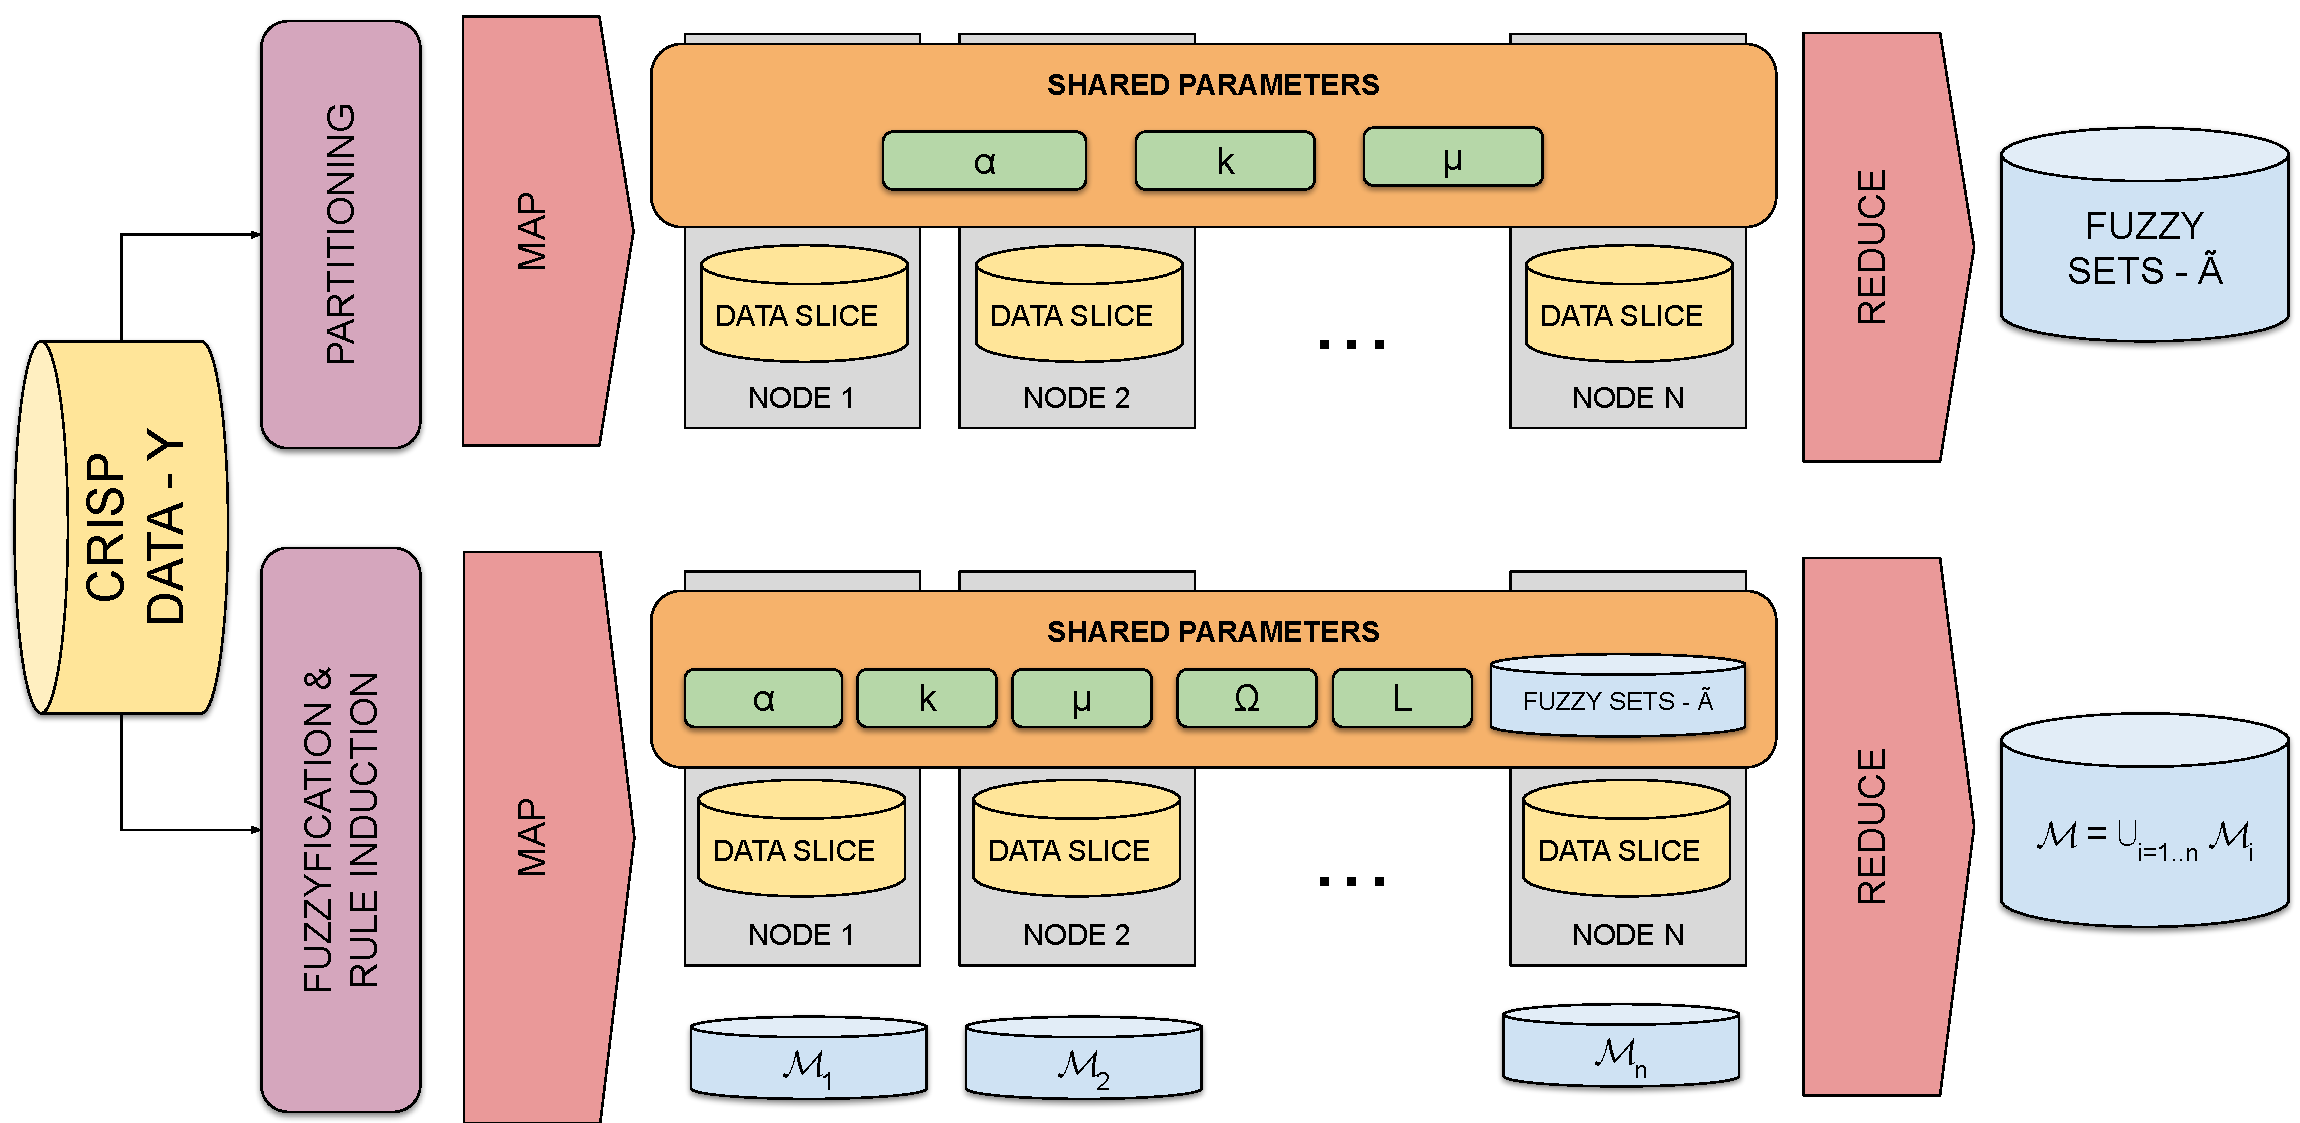
\includegraphics[width=\textwidth]{figures/distributed_models_training.pdf}
    \caption{Training of distributed models}
    \label{fig:distributed_models_training}
\end{figure}

%%%%%%%%%%%%%%%%%%%%%%%%%%%%%%%%%%%%%%%%%%%%%%%%%%%%%%%%%
%%%%%%%%%%%%%%%%%%%%%%%%%%%%%%%%%%%%%%%%%%%%%%%%%%%%%%%%%
\subsubsection{Distributed forecasting procedure}
\label{sec:distributed_forecasting}

The computational cost of the forecasting procedure is low when compared with the training procedure. The forecasting procedure bottlenecks are the fuzzyfication and rule matching steps, and both of them can be optimized using spatial indexes, for instance KD-trees \citep{Muja2014}, which are more efficient when executed locally. Also, as on every distributed procedure, the communication overhead makes this procedure inefficient for data with low volume.

However, there are occasions where the model needs to be used for forecasting in batch, where the input has high volume and one step ahead forecasting will be performed for each data point. This scenario is common in model testing, simulation and hyper-parameter optimization. In these cases it is profitable to share the parameters of the model $\mathcal{M}$ across several slave nodes and perform the forecasting on data splits, keeping its time ordering. The steps of the distributed forecasting procedure are listed below:

 \begin{enumerate}
    \item \textbf{Share}: The linguistic variable $\ulvar$ and the rules $\model$ are shared across the cluster; 
    \item \textbf{Map}: Distribute the $Y$ dataset over the slave nodes, such that each split is labelled with its time ordering;
    \item \textbf{Forecast} Each slave node receives a data split $Y_p$ and executes the sequential forecasting process, generating the estimates $\hat{Y_p}$, sending it back to the master node with the same time label received with $Y_p$;
    \item \textbf{Reduce}: Collect the $\hat{Y_p}$ estimates from the slave nodes;
    \item \textbf{Merge}: Sort the $\hat{Y_p}$ estimates by their time label and concatenate them on a unique dataset $\hat{Y}$.
\end{enumerate}


The proposed distributed methods speed up, or even make possible, to tackle high processing tasks, for instance iterative optimization procedures, using big time series and the previously proposed FTS methods. In next section an adaption of evolutionary algorithm is proposed to FTS hyperparameter optimization. 


%%%%%%%%%%%%%%%%%%%%%%%%%%%%%%%%%%%%%%%%%%%%%%%%%%%%%%%%%
%%%%%%%%%%%%%%%%%%%%%%%%%%%%%%%%%%%%%%%%%%%%%%%%%%%%%%%%%
\section{Distributed Evolutionary Hyperparameter Optimization}
\label{sec:hyperparameter}
\index{Distributed Evolutionary Hyperparameter Optimization}\index{DEHO}

This section aims to propose the Distributed Evolutionary Hyperparameter Optimization - DEHO for FTS methods. The DEHO approach combines the FTS distributed training and forecasting methods with evolutionary optimization algorithms, specifically Genetic Algorithms, in order to optimize FTS models in terms of accuracy and parsimony for big time series.

Given a set of hyperparameters $\Theta$ and an accuracy function $f: \Theta \rightarrow \mathbb{R}^+$, the hyperparameter optimization task aims to discover the values of each hyperparameter $\theta \in \Theta$ such that $\hat{\theta} = \arg\min_\theta f(\Theta)$. The hyperparameter optimization is a computational expensive task and, on a Big Data context, its cost may be prohibitive. The general FTS training procedure does not incorporate any kind of optimization, leaving to the user the task of empirically searching for the best hyperparameters. In the meantime, these parameters have great impact on final model performance and their optimization is highly recommended. At this point, it is necessary to take advantage of the speed up provided by the distributed method in Section \ref{sec:distributed} and to employ an efficient optimization method. 

It is necessary to advise that the partitioning method $\Pi$ was taken out of the optimization, and was kept constant as the Grid Partitioning. The reason is that, besides the Grid Partitioning, the other heuristic and metaheuristic $\Pi$ methods can not be trained with separated data and after merged without compromising its original features. This special aspect must be the subject of future investigations in order to enhance the DEHO method.

Two conflicting goals are sought during the hyperparameter optimization, the accuracy and the parsimony (the structural complexity as usually measured by the number of parameters of the model). In fuzzy time series models, to increase model's accuracy  it is common to increase the number of fuzzy sets $k$ and/or the order $\Omega$ of the model, which automatically increases the number of fuzzy rules $|\model|$. As the number of rules grows, the computational complexity of the model also increases and the FTS approach becomes less interesting when compared with other standard approaches, such as ARIMA or QAR. The challenge is to find a balance between these two objectives, keeping the model small, fast and accurate.

The FTS hyperparameter optimization problem is formulated below, where the objective function $f_1$ \eqref{eqn:hyperopt_f1} controls the accuracy (represented by the weighted sum of the mean error $\bar{\epsilon}$ \eqref{eqn:hyperopt_error_avg} and the standard deviation of the error $\sigma_\epsilon$ \eqref{eqn:hyperopt_error_std}) of the model and the objective function $f_2$ \eqref{eqn:hyperopt_f2} controls for parsimony (represented by the weighted sum of the model length $|\mathcal{M}|$ \eqref{eqn:hyperopt_num_rules} and the sum of the lags $|L|$ \eqref{eqn:hyperopt_lags_sum}). Some additional restrictions are imposed on the order $\Omega$ \eqref{eqn:hyperopt_order}, number of partitions $k$ \eqref{eqn:hyperopt_num_partitions}, $\alpha$-cut \eqref{eqn:hyperopt_alpha_cut}, and the lags indexes $L$ \eqref{eqn:hyperopt_lag_inc}. 

\textbf{Optimize}:
\begin{align}
minimize \quad  f_1  = & \quad 0.6\bar{\epsilon} + 0.4\sigma_\epsilon \label{eqn:hyperopt_f1}\\
minimize \quad  f_2  = & \quad 0.6|\mathcal{M}| + 0.4|L|  \label{eqn:hyperopt_f2}
\end{align}

\textbf{Where:}
\begin{equation}
RMSE = \sqrt{\sum_{t=0}^n (y(t) - \hat{y}(t))^2 )}
 \label{eqn:hyperopt_rmse}
\end{equation}
\begin{align}
\bar{\epsilon} & =  W^{-1}\sum_{i=0}^W RMSE(i) \label{eqn:hyperopt_error_avg} \\
\sigma_\epsilon & =  W^{-1}\sum_{i=0}^W \bar{\epsilon} - RMSE(i)  \label{eqn:hyperopt_error_std}
\end{align}
\begin{align}
|\model| &= \sum_{i=0}^{rules} 1  \label{eqn:hyperopt_num_rules} \\
|L| &= \sum_{i=0}^{\Omega-1} L(i)  \label{eqn:hyperopt_lags_sum} 
\end{align}

\textbf{Subject to}:

\begin{align}
\Omega &\geq 1  \label{eqn:hyperopt_order}\\
k &\geq 3  \label{eqn:hyperopt_num_partitions}\\
\alpha &\in [0,1)  \label{eqn:hyperopt_alpha_cut}\\
1 \leq L(0) & < ... < L(\Omega)  \label{eqn:hyperopt_lag_inc}
\end{align}

Genetic Algorithms (GA) are population-based metaheurisc approaches for solving the optimization problems based on a genetic refinement metaphor. Vanilla GA algorithms are intended for mono-objetive optimization, but with few adaptions it is possible to handle multi-objetive problems as well. In this work the adaptions were made on selection operator, which implements the Double Tournament strategy in order to comprise both objectives on balancing the population.

The set of hyperparameters $\Theta$ is presented in Table \ref{tab:fts_hyperparameters}, except the partitioning method $\Pi$, such that $\Theta = \{\mu,k,\alpha,\Omega,L\}$. Each individual of the population is represented by a vector - the genotype - with the values of each hyperparameter $\theta \in \Theta$. This vector contains both real, categorical and array values, according to hyperparameter type. The GA iterates over steps listed below until the stop criteria is achieved:

\begin{enumerate}
    \item \textbf{Initial Population}: The initial population, with size $NP$, is generated randomly, except for the hyperparameter $L$, whose size is constrained by $\Omega$ and the lag indexes initially consider the most significant ACF/PACF lags.
    
    \item \textbf{Evaluation:} Each genotype is transformed into a trained model - the phenotype - using the distributed method of Section \ref{sec:distributed} and then evaluated. The phenotype evaluation uses the metrics according the objective function $f_1$ and $f_2$ and after the evaluation procedure, the population is sorted by $f_1$ and $f_2$ in ascending order.

    \item \textbf{Selection:} The selection operator is responsible to choose one part of the individuals that will survive for the next generation. As the problem is multi-objective, a Double Tournament strategy was implemented to balance the selection between the two objectives. In the double tournament, the first round chooses randomly two pairs of individuals in the population, and each pair will compete with each other based on objective $f_1$. On the second round the winner individuals of the first round will compete with each other based on the objective $f_2$. This process is repeated by a rate $SR$ of the population.
    
    \item \textbf{Elitism:} As the selection operator is random, there is the possibility that the best individual of the population be discarded. The elitist strategy will keep the best individual of the current generation in the next generation and discard the worst.

    \item \textbf{Crossover:} The crossover operator combines the genotypes of two individuals ($i_1$ and $i_2$) in order to generate a descendent individual ($i_N$). On crossover, two individuals are randomly selected in the population and ordered as $i_1$ and $i_2$ according to their $f_1$ and $f_2$ objectives. For all genes the mixing process will give a major contribution for the best ranked individual (with $.7$ and $.3$ rates). For the real coded genes a linear combination as $i_N = .7i_1 + .3i_2$ will be performed. For the categorical genes, the value of $i_N$ will be $i_1$ with probability $.7$ or $i_2$ otherwise. For the lag $L$ the individual lags will be also a linear combination of each lag. This process is repeated by a rate $CR$ of the population.

    \item \textbf{Mutation:} The mutation operator aims to introduce novelties in the population, then an individual is randomly chosen and random perturbations are applied to its genes, taking care to keep the gene values feasible according to the problem restrictions. This process is repeated by a rate $MR$ of the population.

    \item \textbf{Stop Criteria:} Repeat the steps 2 to 7 until one of these criteria are achieved: $NG_{stop}$ generations without improvement or maximum number of generations $NG$.
\end{enumerate}

This Genetic Algorithm requires the choice of the  parameters presented in Table \ref{tab:genetic_algoritm}. The complete hyper-parameter optimization method also requires the choosing of the distribution type and the parameters presented in Table \ref{tab:distributed_testing}.

\begin{table}[htb]
    \centering
    \begin{tabular}{|c|p{7cm}|} \hline
        \textbf{Parameter} & \textbf{Description}  \\ \hline
         $PS \in \mathbb{N}^+$ & Population Size \\ \hline
         $NG \in \mathbb{N}^+$ & Max Number of Generations \\ \hline 
         $0 < NG_{stop} < NG$ & Max Number of Generations without improvement \\ \hline 
         $SR \in [0,1]$ & Selection Rate \\ \hline 
         $CR \in [0,1]$ & Crossover Rate \\ \hline 
         $MR \in [0,1]$ & Mutation Rate \\ \hline 
    \end{tabular}
    \caption{Genetic Algorithm parameters}
    \label{tab:genetic_algoritm}
\end{table}

%%%%%%%%%%%%%%%%%%%%%%%%%%%%%%%%%%%%%%%%%%%%%%%%%%%%%%%%%
%%%%%%%%%%%%%%%%%%%%%%%%%%%%%%%%%%%%%%%%%%%%%%%%%%%%%%%%%

\section{Computational Experiments}
\label{sec:scalability_experiments}

This section presents an exploratory study of distributed models performance and the DEHO method. The computational experiments employed a large sized environmental time series, the SONDA dataset with 2,000,000 instances, and a medium sized time series, the Malaysia dataset, with 17,000 instances. Both datasets are detailed in Appendix \ref{apd:multivariate_datasets}, where its main characteristics are presented.

In Section \ref{sec:scalability_speedup} the speed ups provided by the distributed training and forecasting are presented by several cluster configurations. In \ref{sec:scalability_convergence} the distributed methods are employed in DEHO method, and the convergence of the method is analyzed.

In order to contribute with the replication of all the results in the research, all data and source codes employed in this chapter are available at the URL:
\texttt{\url{http://bit.ly/scalable_probabilistic_fts_chap5}}

%%%%%%%%%%%%%%%%%%%%%%%%%%%%%%%%%%%%%%%%%%%%%%%%%%%%%%%%%
%%%%%%%%%%%%%%%%%%%%%%%%%%%%%%%%%%%%%%%%%%%%%%%%%%%%%%%%%
\subsection{Speed Up Of Distributed Methods}
\label{sec:scalability_speedup}

In order to assess the impact of including more processing nodes on training and forecasting processing times of distributed methods, different cluster configurations were evaluated .

The performance of the sequential and distributed methods, on above cited clusters configurations, was measured in terms of execution time (in seconds) and the speed up from the sequential time, such that $S_p = \frac{T_1}{T_p}$, where $S_p$ is the speed up for $p$ nodes, $T_1$ is the time of the sequential execution and $T_p$ is the time of the distributed execution with $p$ nodes. 

The experiments show improvements on performance for each added node on the large sized dataset, but this improvement is smaller in the medium sized dataset.  The trade-off between the distribution overhead and the benefit of the distributed computations stops to be profitable above the third node on the cluster for medium sized datasets. Above 3 nodes the network overhead for the length of data makes the distributed algorithm not interesting. However, it can be seen that an average speed up of 2x was achieved on the training procedure for large time series, showing that the performance tends to increase on more robust computational clusters.  


\begin{table}[ht]
\resizebox{\textwidth}{!}{% <------ Don't forget this %
    \centering
    \begin{tabular}{|c|c|c|c|c|c|} \hline
        Dataset & CPU's 
        & \begin{tabular}{c} Training \\ Time \end{tabular} 
        & \begin{tabular}{c} Training \\ Speed Up \end{tabular}
        & \begin{tabular}{c} Forecasting \\ Time  \end{tabular}
        & \begin{tabular}{c} Forecasting \\ Speed Up \end{tabular}  \\ \hline
        \multirow{7}{*}{SONDA Wind Speed} 
             & 1 & 685.25 $\pm$ 135.16 & - & 285.89 $\pm$ 57.94 & - \\ \cline{2-6}
             & 2 & 383.29 $\pm$ 72.50 & 1.78 & 164.82 $\pm$ 30.10 & 1.73 \\ \cline{2-6}
             & 3 & 330.13 $\pm$ 64.55 & 2.07 & 138.58 $\pm$ 25.37 & 2.06 \\ \cline{2-6}
             & 4 & 342.64 $\pm$ 52.86 & 1.99 & 151.34 $\pm$ 25.54 & 1.88 \\ \cline{2-6}
             & 5 & 300.75 $\pm$ 58.19 & 2.27 & 130.67 $\pm$ 23.20 & 2.18 \\ \cline{2-6}
             & 6 & 348.98 $\pm$ 67.41 & 1.96 & 153.16 $\pm$ 30.0 & 1.86 \\ \cline{2-6}
             & 7 & 361.45 $\pm$ 65.61 & 1.89 & 160.74 $\pm$ 30.68 & 1.77 \\ \hline
        \multirow{7}{*}{SONDA Solar Radiation }
             & 1 & 651.29 $\pm$ 121.95 & - & 274.28 $\pm$ 47.72 & - \\ \cline{2-6}
             & 2 & 383.24 $\pm$ 66.37 & 1.69 & 165.98 $\pm$ 36.21 & 1.65 \\ \cline{2-6}
             & 3 & 314.10 $\pm$ 59.98 & 2.07 & 136.92 $\pm$ 24.63 & 2.00 \\ \cline{2-6}
             & 4 & 345.55 $\pm$ 64.135 & 1.88 & 152.31 $\pm$ 28.43 & 1.8 \\ \cline{2-6}
             & 5 & 289.38 $\pm$ 54.44 & 2.25 & 129.52 $\pm$ 24.22 & 2.11 \\ \cline{2-6}
             & 6 & 340.35 $\pm$ 59.64 & 1.91 & 153.09 $\pm$ 28.35 & 1.79 \\ \cline{2-6}
             & 7 & 349.70 $\pm$ 65.48 & 1.86 & 159.16 $\pm$ 28.46 & 1.72 \\ \hline
        \multirow{7}{*}{Malaysia Temperature }
             & 1 & 12.28 $\pm$ 0.70 & - & 5.11 $\pm$ 0.35 & - \\ \cline{2-6}
             & 2 & 7.21 $\pm$ 0.48 & 1.7 & 3.42 $\pm$ 0.23 & 1.49 \\ \cline{2-6}
             & 3 & 6.64 $\pm$ 0.45 & 1.84 & 3.24 $\pm$ 0.24 & 1.57 \\ \cline{2-6}
             & 4 & 7.44 $\pm$ 0.18 & 1.64 & 3.95 $\pm$ 0.23 & 1.29 \\ \cline{2-6}
             & 5 & 6.56 $\pm$ 0.29 & 1.87 & 3.93 $\pm$ 0.47 & 1.30 \\ \cline{2-6}
             & 6 & 7.46 $\pm$ 0.24 & 1.64 & 4.44 $\pm$ 0.23 & 1.15 \\ \cline{2-6}
             & 7 & 8.09 $\pm$ 0.27 & 1.51 & 5.15 $\pm$ 0.01 & 0.99 \\ \hline
        \multirow{7}{*}{Malaysia Load }
             & 1 & 13.05 $\pm$ 1.50 & - & 5.32 $\pm$ 0.59 & - \\ \cline{2-6}
             & 2 & 7.84 $\pm$ 0.9 & 1.66 & 3.43 $\pm$ 0.24 & 1.54 \\ \cline{2-6}
             & 3 & 7.14 $\pm$ 0.75 & 1.82 & 3.42 $\pm$ 0.21 & 1.55 \\ \cline{2-6}
             & 4 & 8.06 $\pm$ 1.01 & 1.61 & 4.31 $\pm$ 0.39 & 1.23 \\ \cline{2-6}
             & 5 & 8.18 $\pm$ 2.31 & 1.59 & 4.10 $\pm$ 0.41 & 1.29 \\ \cline{2-6}
             & 6 & 8.06 $\pm$ 1.01 & 1.61 & 4.77 $\pm$ 0.46 & 1.11 \\ \cline{2-6}
             & 7 & 8.90 $\pm$ 0.86 & 1.46 & 6.18 $\pm$ 0.71 & 0.86 \\ \hline
    \end{tabular}
    }
    \caption{Speed up provided by the distributed model by number of CPU's}
    \label{tab:speed_up}
\end{table}

\begin{figure}
    \centering
    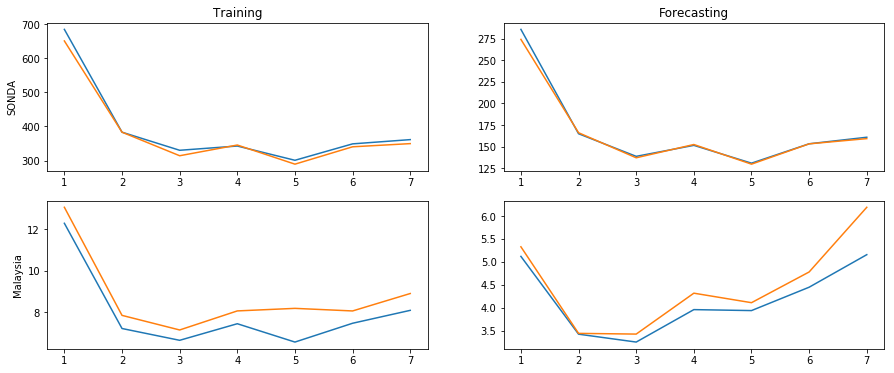
\includegraphics[width=\textwidth]{figures/speed_up.png}
    \caption{Speed up provided by the distributed model by number of CPU's}
    \label{fig:speed_up}
\end{figure}

%%%%%%%%%%%%%%%%%%%%%%%%%%%%%%%%%%%%%%%%%%%%%%%%%%%%%%%%%
%%%%%%%%%%%%%%%%%%%%%%%%%%%%%%%%%%%%%%%%%%%%%%%%%%%%%%%%%
\subsection{Convergence of DEHO approach}
\label{sec:scalability_convergence}

The DEHO method was employed using a computational cluster with 7 CPU's and the parameters contained in Table \ref{tab:hyperopt_parameters} using PWFTS as FTS method. The experiment performed 5 executions of DEHO for each dataset and the averaged results are presented in Table \ref{tab:hyperopt_results}. A sample of the convergence process of DEHO can be seen in Figure \ref{fig:deho_convergence}, for  SONDA Wind Speed dataset. 

The results showed that, for the studied time series, the convergence was fast, expending about 16 generations on average. In the trade off between the objectives $f_1$ and $f_2$, the accuracy objective showed to be predominant over the parsimony objective during the convergence of the method. 

The optimized values for the hyperparameters generated parsimonic and accurated forecasting models, whose samples of their performance can be seen in Figure

\begin{table}[htb]
    \centering
    \begin{tabular}{|c|c|c|} \hline
        \textbf{Parameter} & \textbf{Dataset} & \textbf{Value} \\ \hline
         \multirow{4}{*}{$W_L$}  & 
         \begin{tabular}{c}
              SONDA  \\
              Wind Speed 
         \end{tabular} & 600,000 \\ \cline{2-3}
                & 
        \begin{tabular}{c}
              SONDA  \\
              Solar Radiation  
         \end{tabular} & 600,000 \\ \cline{2-3}
                & 
        \begin{tabular}{c}
              Malaysia  \\
              Temperature  
         \end{tabular} & 10,000 \\ \cline{2-3}
                & 
        \begin{tabular}{c}
              Malaysia  \\
              Eletric Load  
         \end{tabular} & 10,000 \\ \hline
         $W_I$ & All &  .5 \\ \hline
         $T_S$ &  All &.9  \\ \hline
         $PS$ &  All &20  \\ \hline
         $NG$ &  All &30  \\ \hline 
         $NG_{stop}$  &  All &10  \\ \hline 
         $SR$ &  All &.5  \\ \hline 
         $CR$ &  All &.5  \\ \hline 
         $MR$ &  All &.2  \\ \hline  
    \end{tabular}
    \caption{Distributed Evolutive Hyperparameter Optimization parameter values}
    \label{tab:hyperopt_parameters}
\end{table}


\begin{table}[htb]
\resizebox{\textwidth}{!}{% <------ Don't forget this %
\begin{tabular}{|c|c|c|c|c|c|c|c|c|}
\hline
\textbf{Dataset}                       & \textbf{Generations}                                                            & $\mathbf{k}$                                                                   & $\mathbf{\mu}$     & $\mathbf{\alpha}$                                                              & $\mathbf{\Omega}$  & $\mathbf{L}$               & \textbf{Metric} & \textbf{Value}                                                  \\ \hline
\multirow{3}{*}{SONDA Solar Radiation} & \multirow{3}{*}{\begin{tabular}[c]{@{}c@{}}16.4 \\ $\pm$ 7.8\end{tabular}}      & \multirow{3}{*}{\begin{tabular}[c]{@{}c@{}}50.8 \\ $\pm$ 0.7\end{tabular}}  & \multirow{3}{*}{2} & \multirow{3}{*}{\begin{tabular}[c]{@{}c@{}}0.24 \\ $\pm$ 0.13\end{tabular}} & \multirow{3}{*}{2} & \multirow{3}{*}{{[}1,2{]}} & $|\model|$      & 613 $\pm$ 222     \\ \cline{8-9} 
                                       &                                                                                 &                                                                                &                    &                                                                                &                    &                            & RMSE            & 93.13 $\pm$ 0.62  \\ \cline{8-9} 
                                       &                                                                                 &                                                                                &                    &                                                                                &                    &                            & Time            & 3221 $\pm$ 1505   \\ \hline
\multirow{3}{*}{SONDA Wind Speed} & \multirow{3}{*}{30.0}      & \multirow{3}{*}{50}  & \multirow{3}{*}{1} & \multirow{3}{*}{\begin{tabular}[c]{@{}c@{}}0.13 \\ $\pm$ 0.1\end{tabular}} & \multirow{3}{*}{1} & \multirow{3}{*}{{[}1{]}} & $|\model|$      & 24 $\pm$ 1.45     \\ \cline{8-9} 
                                       &                                                                                 &                                                                                &                    &                                                                                &                    &                            & RMSE            & 0.34 $\pm$ 74e-10$^{-4}$  \\ \cline{8-9} 
                                       &                                                                                 &                                                                                &                    &                                                                                &                    &                            & Time            & 3058 $\pm$ 891   \\ \hline
\multirow{3}{*}{Malaysia Energy Load}  & \multirow{3}{*}{\begin{tabular}[c]{@{}c@{}}12.5 \\ $\pm$ 2.5\end{tabular}}   & \multirow{3}{*}{\begin{tabular}[c]{@{}c@{}}50.6 \\ $\pm$ 1.2\end{tabular}}  & \multirow{3}{*}{2} & \multirow{3}{*}{\begin{tabular}[c]{@{}c@{}}0.22 \\ $\pm$ 0.23\end{tabular}} & \multirow{3}{*}{2} & \multirow{3}{*}{{[}1,2{]}} & $|\model|$      & 306.9 $\pm$ 137.9 \\ \cline{8-9} 
                                       &                                                                                 &                                                                                &                    &                                                                                &                    &                            & RMSE            & 2745.5 $\pm$ 271.27                                             \\ \cline{8-9} 
                                       &                                                                                 &                                                                                &                    &                                                                                &                    &                            & Time            & 3945.09 $\pm$ 800.71                                            \\ \hline
\multirow{3}{*}{Malaysia Temperature}  & \multirow{3}{*}{\begin{tabular}[c]{@{}c@{}}16.6 \\ $\pm$ 10.15\end{tabular}} & \multirow{3}{*}{\begin{tabular}[c]{@{}c@{}}52.8 \\ $\pm$ 3.18\end{tabular}} & \multirow{3}{*}{1} & \multirow{3}{*}{\begin{tabular}[c]{@{}c@{}}0.24 \\ $\pm$ 0.09\end{tabular}} & \multirow{3}{*}{1} & \multirow{3}{*}{{[}1{]}}   & $|\model|$      & 73.21 $\pm$ 1.08                                                \\ \cline{8-9} 
                                       &                                                                                 &                                                                                &                    &                                                                                &                    &                            & RMSE            & 1.08 $\pm$ 0.06                                                 \\ \cline{8-9} 
                                       &                                                                                 &                                                                                &                    &                                                                                &                    &                            & Time            & 3916.58 $\pm$ 2042.12                                           \\ \hline
\end{tabular}
}
\caption{Optimization mean results by dataset}
\label{tab:hyperopt_results}
\end{table}

\begin{figure}[htb]
    \centering
    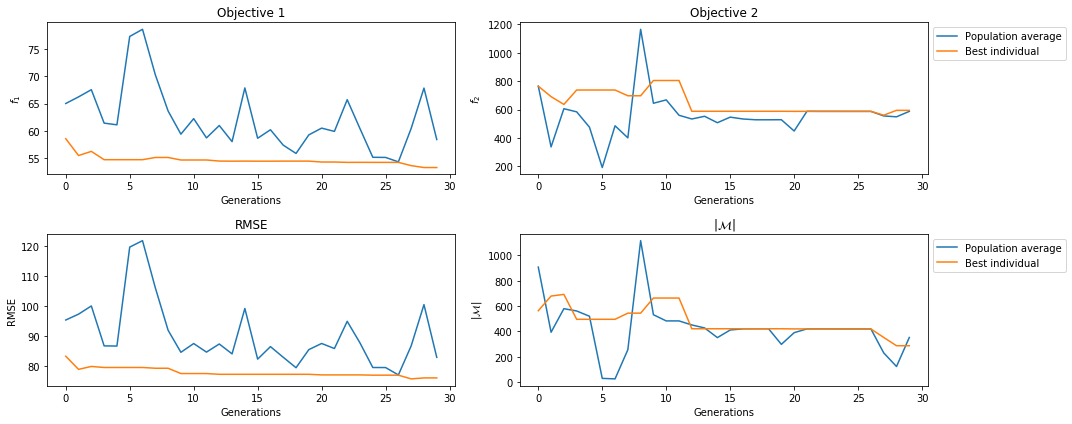
\includegraphics[width=\textwidth]{figures/deho_convergence.png}
    \caption{Sample of DEHO convergence}
    \label{fig:deho_convergence}
\end{figure}

%%%%%%%%%%%%%%%%%%%%%%%%%%%%%%%%%%%%%%%%%%%%%%%%%%%%%%%%%
%%%%%%%%%%%%%%%%%%%%%%%%%%%%%%%%%%%%%%%%%%%%%%%%%%%%%%%%%
\section{Conclusion}
\label{sec:scalability_conclusion}

Training accurate models for forecasting big time series is a challenging task for traditional and soft-computing methods. Usually the methods are not designed to deal with such high volume of data. When such data volume cannot be grounded on a single machine memory, it demands a distributed architecture of storage and processing. This is particularly problematic when optimizing the hyperparameters of a method, because successive model training and testing processes are required. 

This chapter proposed two distributed approaches for FTS model scalability, one for middle sized data and another for big sized data. The first one distributes the data across the nodes of a cluster, where individual models are trained and tested. The second one, the distributed model itself, splits the training of a unique model across several nodes, allowing a big time series model to be trained in pieces and then aggregated into a single model.

These approaches were employed on Distributed Evolutionary Hyperparameter Optimization (DEHO). DEHO method is an adapted genetic algorithm that minimizes two cost functions, the accuracy function $f_1$ and the parsimony function $f_2$. An exploratory study was performed in order to measure the feasibility of the proposed distributed models and showed the speed-up provided for big time series. The convergence of DEHO method also was analyzed, showing its effectiveness.

\subsection{Method limitations}

The distributed training method is indicated only for big time series. Using the method for small data might slow down the training time due to the network and model merging overheads. DEHO method took into account only time invariant, rule based, monovariate and high-order methods, not being applicable for time variant, multivariate and first order FTS methods.  

Next chapter presents a short review of multivariate methods and proposes a simple approach for extending PWFTS to forecasting multivariate time series.

